%!TEX root = ../thesis.tex
%*******************************************************************************
%****************************** Metodologia *********************************
%*******************************************************************************


\chapter{Metodología}\label{chap:metod}

Este trabajo aplica una metodología de \textbf{integración continua y desarrollo colaborativo} de acuerdo con los objetivos del proyecto SIOSE-INNOVA para la implementación de \textit{pg\_landmetrics}.


\section{Integración continua y desarrollo colaborativo}

\begin{graybox}
\begin{itemize}
\item El trabajo colaborativo se ha coordinado utilizando \textit{Git} que es el sistema de \textbf{control de versiones} más popular de los últimos años (p.ej. utilizado en , PostGIS, QGIS, CARTO y decenas de proyectos ESRI, entre muchos otros).
\item La \textbf{contenerización o \textit{dockers}} es una novedosa tecnología para la virtualización de software/servicios, frente a la virtualización de sistemas operativos (p.ej. máquinas virtuales). La orquestación de \textit{dockers} permite organizar complejos sistemas de información con muchas facilidades.
\item PostgreSQL/PostGIS es la \textit{geodatabase libre} más potente del mercado, destacando por sus opciones de \textbf{extensibilidad} (p.ej. PostGIS en sí misma es una extensión de PostgreSQL).
\end{itemize}
\end{graybox}



\subsection{Control de versiones}



\begin{itemize}
\item\textbf{Git}: 
\item\textbf{GitHub}: 
\end{itemize}



\begin{figure}
\begin{center}
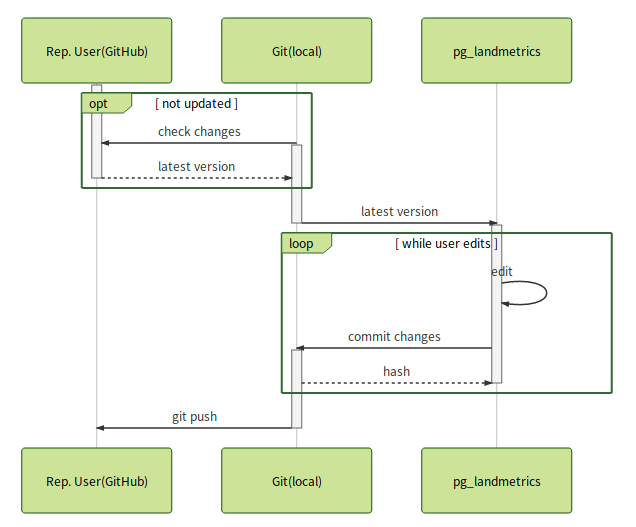
\includegraphics[width=0.9\textwidth]{Metodologia/Figs/diary.png}
\caption{Flujo de proceso de actualización de ficheros. \label{fig:diary}}
\end{center}
\end{figure}



\begin{figure}
\begin{center}
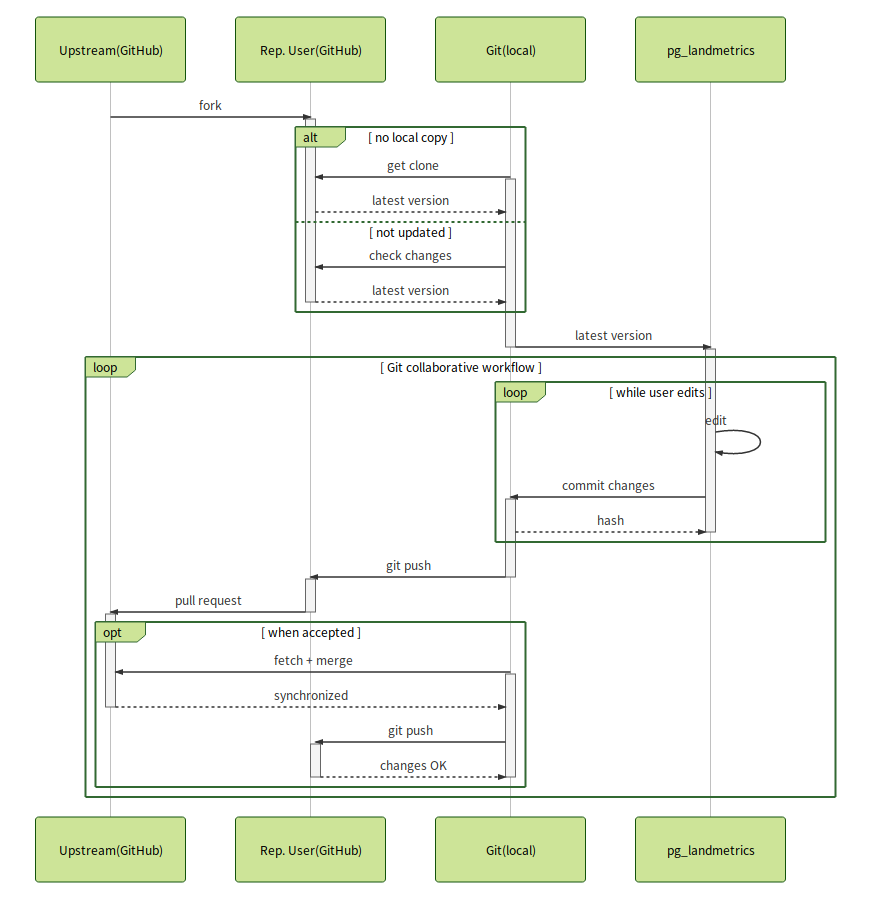
\includegraphics[width=0.9\textwidth]{Metodologia/Figs/pullrequest.png}
\caption{Flujo de proceso de trabajo colaborativo entre repositorios. \label{fig:pullrequest}}
\end{center}
\end{figure}


\subsection{Contenerización y orquestación de servicios}





Se han utilizado los siguientes elementos:
\begin{itemize}
\item\textbf{Docker}: 
\item\textbf{Docker Hub}: 
\item\textbf{Docker-compose}: 
\end{itemize}




\begin{figure}
\begin{center}
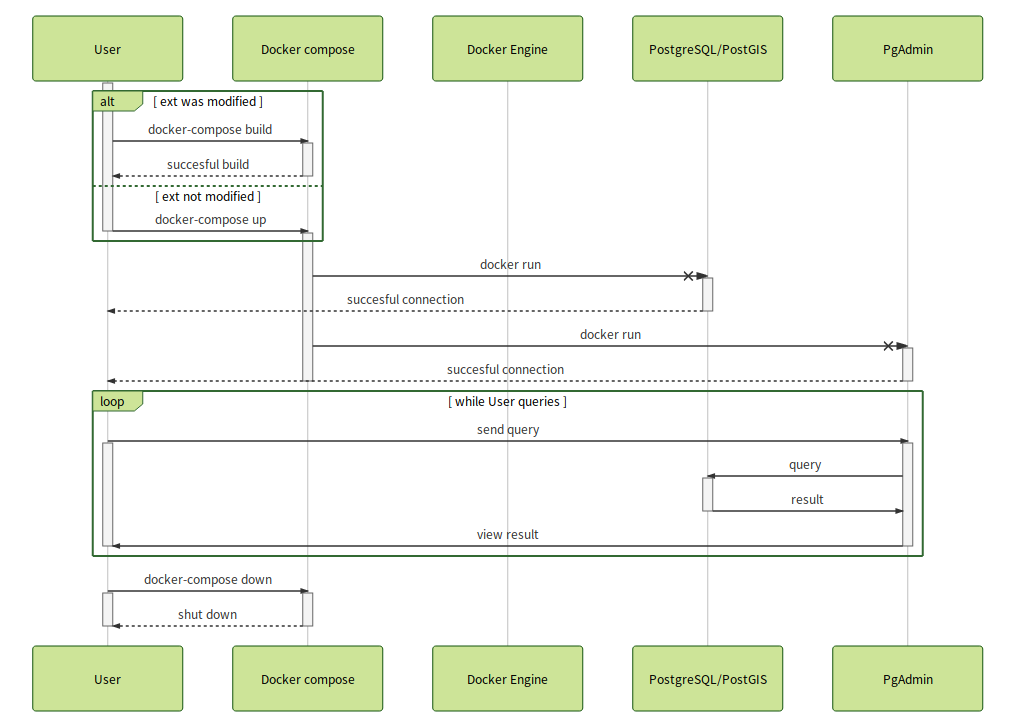
\includegraphics[width=\textwidth]{Metodologia/Figs/ci.png}
\caption{Flujo de proceso de integración continua. \label{fig:ci}}
\end{center}
\end{figure}


\subsection{Extensibilidad}



\begin{itemize}
\item\textbf{PostgreSQL/PostGIS}: 
\end{itemize}

\subsection{Aplicaciones}



\begin{itemize}
\item\textbf{PgAdmin4}: 

\begin{figure}
\begin{center}
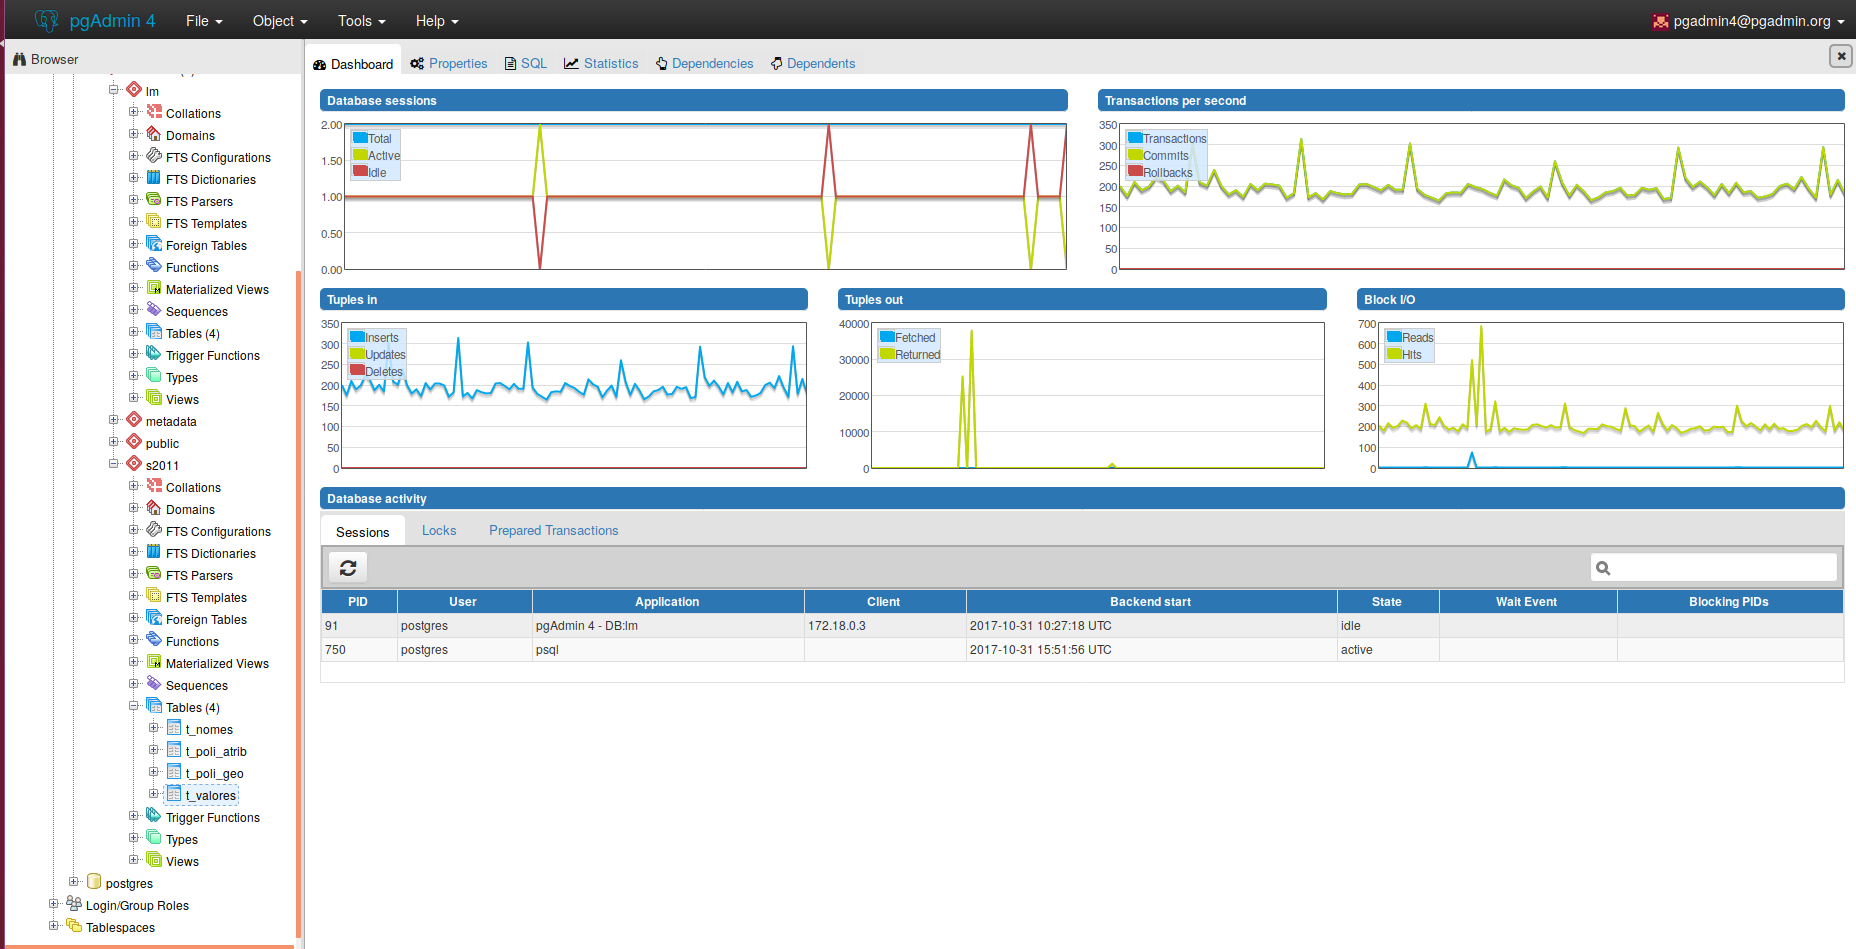
\includegraphics[width=\textwidth]{Metodologia/Figs/carga-siose-2011.png}
\caption{Flujo de proceso de integración continua. \label{fig:carga}}
\end{center}
\end{figure}

\item\textbf{QGIS 2.18}: 
\end{itemize}

\section{Conjunto de datos}

\begin{graybox}
\begin{itemize}
\item En este trabajo se han utilizado dos conjuntos de datos, \textbf{un paisaje de ejemplo y el SIOSE de 2011 completo}, para poner a prueba la extensión \textit{pg\_landmetrics} propuesta en los objetivos.
\end{itemize}
\end{graybox}



\begin{figure}
\begin{center}
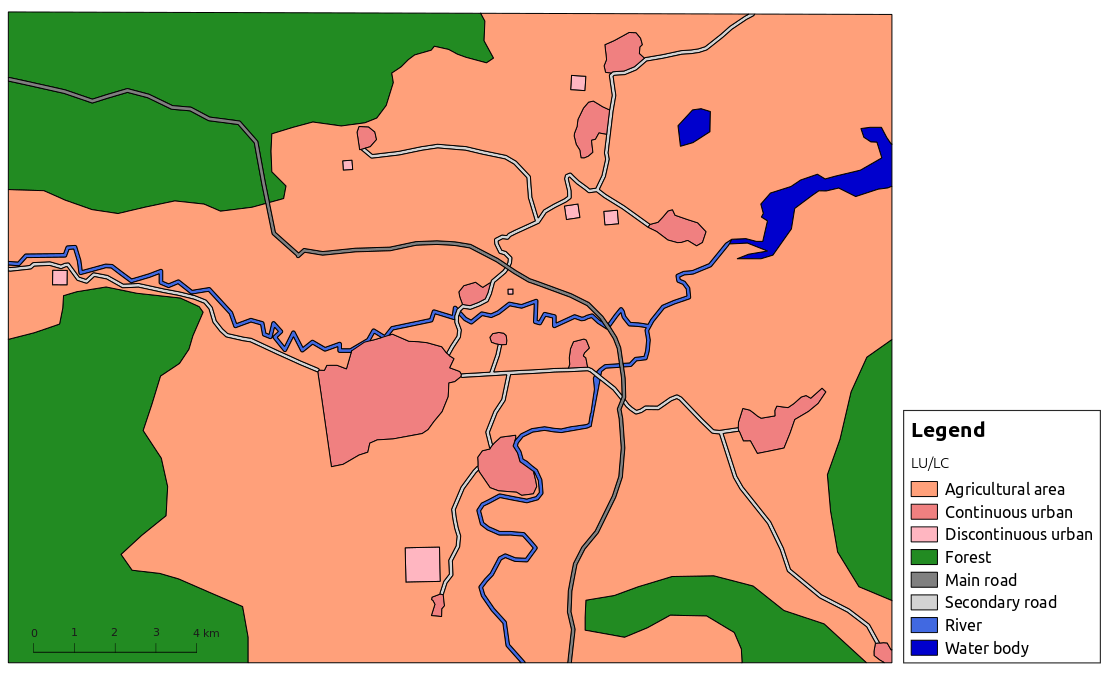
\includegraphics[width=\textwidth]{Metodologia/Figs/land_test.png}
\caption{Uso y cobertura del suelo del paisaje de ejemplo. \label{fig:lan_test}}
\end{center}
\end{figure}

% Please add the following required packages to your document preamble:
% \usepackage{booktabs}
\begin{table}[]
\centering
\caption{Atributos del primer conjunto de datos.}
\label{my-label}
\begin{tabular}{@{}lll@{}}
\toprule
\textbf{Nombre} & \textbf{Tipo de campo}   & \textbf{Descripción}                    \\ \midrule
gid             & integer                  & Identificador único de cada polígono    \\
geom            & geometry                 & Geometría del polígono                  \\
category        & character varying (text) & Clasificación de la cobertura del suelo \\
svg\_color      & character varying (text) & Color según tipo de categoría           \\ \bottomrule
\end{tabular}
\end{table}




\begin{table}[]
\centering
\caption{Color SVG según el tipo de categoría al que corresponde.}
\label{my-label}
\begin{tabular}{ll}
\hline
\textbf{Category}   & \textbf{svg\_color} \\ \hline
Agricultural area   & lightsalmon         \\
Continuous urban    & lightcoral          \\
Discontinuous urban & lightpink           \\
Forest              & forestgreen         \\
Main road           & gray                \\
Secondary road      & lightgrey           \\
River               & royalblue           \\
Water body          & mediumblue          \\ \hline
\end{tabular}
\end{table}



% Please add the following required packages to your document preamble:
% \usepackage{booktabs}
% \usepackage{multirow}
\begin{table}[]
\centering
\caption{Tablas usadas para \textit{pg\_landmetrics}.}
\label{my-label}
\begin{tabular}{@{}llll@{}}
\toprule
\textbf{Tipo}               & \textbf{Tablas} & \textbf{Filas} & \textbf{Tamaño total} \\ \midrule
\multirow{4}{*}{Relational} & t\_nomes        & 36.790.972     & 6116 MB               \\
                            & t\_poli\_atrib  & 2.562.800      & 451 MB                \\
                            & t\_poli\_geo    & 2.562.800      & 3981 MB               \\
                            & t\_valores      & 10.932.639     & 1041 MB               \\ \midrule
\multirow{4}{*}{Grids}      & g25k            & 756            & 232,3 kB              \\
                            & g50k            & 192            & 57,8 kB               \\
                            & g100k           & 48             & 13,8 kB               \\
                            & g500k           & 2              & 677bytes              \\ \bottomrule
\end{tabular}
\end{table}





\section{Selección de métricas}

\begin{graybox}
\begin{itemize}
\item El número potencial de métricas del paisaje es indeterminado y depende de muchos factores (p.ej. objetivos del estudio, modelos de datos como \textit{raster/vector} o en red, niveles de agregación y/o escala, etc).
\item Resulta esencial determinar unas \textbf{métricas representativas} para esta primera propuesta.
\end{itemize}
\end{graybox}

Como se indica en la sección \ref{sec:metrica}, existen cientos de métricas de paisaje que no siempre tienen significado para todas las aplicaciones de estudio ya que dependen de muchos factores, como por ejemplo los objetivos del estudio, el modelo de datos, la escala, nivel de agregación etc. Por este mismo motivo y según los objetivos específicados en este trabajo y en el proyecto SIOSE-INNOVA, se han seleccionado unas determinadas métricas de paisaje.

En la tabla \ref{tab:listmetricas} se aprecian las métricas, acompañadas por su abreviatura, que se han escogido divididas en tres niveles de agregación: a nivel polígono (\textit{patch}), nivel categoría (\textit{class}) y nivel paisaje (\textit{landscape}). Para ello se ha seleccionado un número equitativo entre los niveles de agregación. Además, se han querido escoger algunas métricas que calculen operaciones simples como por ejemplo el área o perímetro, y por otro lado, métricas cuyos cálculos sean más complejos como por ejemplo la distancia del vecino más próximo o la densidad, entre otros.

% Please add the following required packages to your document preamble:
% \usepackage{multirow}
\begin{table}[]
\centering
\caption{Listado de métricas de paisaje disponibles en la extensión.}
\label{tab:listmetricas}
\begin{tabular}{lll}
\hline
\textbf{Nivel}             & \textbf{Métrica}                     & \textbf{Abreviatura} \\ \hline
\multirow{8}{*}{Patch}     & Patch Area                           & AREA                 \\
                           & Patch Perimeter                      & PERIM                \\
                           & Perimeter-Area-Ratio                 & PARA                 \\
                           & Shape Index                          & SHAPE                \\
                           & Core Area                            & CORE                 \\
                           & Number of Core Areas                 & NCORE                \\
                           & Core Area Index                      & CAI                  \\
                           & Euclidean Nearest Neighbour Distance & ENN                  \\ \hline
\multirow{8}{*}{Class}     & Total (Class) Area                   & CA                   \\
                           & Percentage of Landscape              & PLAND                \\
                           & Total Edge                           & TE                   \\
                           & Edge Density                         & ED                   \\
                           & Total Core Area                      & TCA                  \\
                           & Core Area Percentage of Landscape    & CPLAND               \\
                           & Number of Patches                    & NP                   \\
                           & Patch Density                        & PD                   \\ \hline
\multirow{9}{*}{Landscape} & Total Area                           & TA                   \\
                           & Total Edge                           & TE                   \\
                           & Edge Density                         & ED                   \\
                           & Number of Patches                    & NP                   \\
                           & Patch Density                        & PD                   \\
                           & Patch Richness                       & PR                   \\
                           & Patch Richness Density               & PRD                  \\
                           & Shannon's Diversity Index            & SHDI                 \\
                           & Simpson's Diversity Index            & SHIDI                \\ \hline
\end{tabular}
\end{table}


\section{Implementación/desarrollo de funciones en PostgreSQL}

\begin{graybox}
\begin{itemize}
\item Los desarrollos en PostgreSQL se pueden realizar en lenguajes de programación como ANSI C, SQL y/o distintos lenguajes procedurales (p.ej. PLpgSQL, PL/R, PL/Python, entre muchos otros), \textbf{dependiendo de las necesidades}.
\end{itemize}
\end{graybox}

% Please add the following required packages to your document preamble:
% \usepackage{booktabs}
% \usepackage{multirow}
\begin{table}[]
\centering
\caption{My caption}
\label{my-label}
\begin{tabular}{@{}lllll@{}}
\toprule
\textbf{id} & \textbf{level}              & \textbf{s\_name} & \textbf{l\_name}                     & \textbf{unit\_id} \\ \midrule
1           & \multirow{8}{*}{Patch}      & AREA             & Patch Area                           & 1                 \\
2           &                             & PERIM            & Patch Perimeter                      & 2                 \\
3           &                             & PARA             & Perimeter Area Ratio                 & 3                 \\
4           &                             & SHAPE            & Shape Index                          & 5                 \\
5           &                             & CORE             & Core Area                            & 1                 \\
6           &                             & NCORE            & Number of Core Area                  & 5                 \\
7           &                             & CAI              & Core Area Index                      & 4                 \\
8           &                             & ENN              & Euclidean Nearest Neighbour Distance & 2                 \\ \midrule
9           & \multirow{8}{*}{Class}      & CA               & Total (Class) Area                   & 1                 \\
10          &                             & PLAND            & Percentage of Landscape              & 4                 \\
11          &                             & TE               & Total Edge                           & 2                 \\
12          &                             & ED               & Edge Density                         & 6                 \\
13          &                             & TCA              & Total Core Area                      & 1                 \\
14          &                             & CPLAND           & Core Area Percentage of Landscape    & 4                 \\
15          &                             & NP               & Number of Patches                    & 5                 \\
16          &                             & PD               & Patch Density                        & 7                 \\ \midrule
17          & \multirow{9}{*}{Landscape}  & TA               & Total Area                           & 1                 \\
18          &                             & TE               & Total Edge                           & 5                 \\
19          &                             & ED               & Edge Density                         & 6                 \\
20          &                             & NP               & Number of Patches                    & 5                 \\
21          &                             & PD               & Patch Density                        & 7                 \\
22          &                             & PR               & Patch Richness                       & 5                 \\
23          &                             & PRD              & Patch Richness Density               & 7                 \\
24          &                             & SHDI             & Shannon's Diversity Index            & 5                 \\
25          &                             & SHIDI            & Simpson's Diversity Index            & 5                 \\ \midrule
26          & \multirow{2}{*}{Proportion} & PC               & Proportion Class                     & 4                 \\
27          &                             & PL               & Proportion Landscape                 & 4                 \\ \bottomrule
\end{tabular}
\end{table}

% Please add the following required packages to your document preamble:
% \usepackage{booktabs}
\begin{table}[]
\centering
\caption{My caption}
\label{my-label}
\begin{tabular}{@{}lll@{}}
\toprule
\textbf{id\_unit} & \textbf{s\_unit} & \textbf{l\_unit}         \\ \midrule
1                 & Ha.              & Hectáreas                \\
2                 & m.               & Metros                   \\
3                 & m²               & Metros cuadrados         \\
4                 & \%               & Porcentaje               \\
5                 & -                & Ninguno                  \\
6                 & m/Ha             & Metros por Hectárea      \\
7                 & num/100 Ha       & Número por 100 Hectáreas \\ \bottomrule
\end{tabular}
\end{table}

\lstset{caption=Crear una función para calcular el IDW (I),label= IDW1}
\begin{SQL}
SELECT St_Area(geom)/10000 FROM sample_patches_25830;
SELECT St_Area(geom)/10000 FROM sample_patches_4326;
\end{SQL}

\lstset{caption=Crear una función para calcular el IDW (I),label= IDW1}
\begin{SQL}
SELECT SUM(St_Area(geom))/10000, category FROM sample_patches_25830 GROUP BY category;
SELECT SUM(St_Area(geom))/10000, category FROM sample_patches_4326 GROUP BY category;
\end{SQL}

\lstset{caption=Crear una función para calcular el IDW (I),label= IDW1}
\begin{SQL}
SELECT SUM(St_Area(geom)) FROM sample_patches_25830;
SELECT SUM(St_Area(geom)) FROM sample_patches_4326;
\end{SQL}


\lstset{caption=Crear una función para calcular el IDW (I),label= IDW1}
\begin{SQL}
SELECT St_Distance(p1.geom, p2.geom) 
FROM sample_patches_25830 AS p1, sample_patches_25830 AS p2
WHERE p1.id = 1 AND p1.id <> p2.id AND p2.category= "category"
ORDER BY St_Distance (p1.geom, p2.geom)
LIMIT 1;

SELECT St_Distance(p1.geom, p2.geom) 
FROM sample_patches_4326 AS p1, sample_patches_4326 AS p2
WHERE p1.id = 1 AND p1.id <> p2.id AND p2.category= "category"
ORDER BY St_Distance (p1.geom, p2.geom)
LIMIT 1;
\end{SQL}

\lstset{caption=Crear una función para calcular el IDW (I),label= IDW1}
\begin{SQL}
SELECT SUM(St_Area(St_Buffer(geom, -100)))/10000 FROM sample_patches_25830 GROUP BY category;
SELECT SUM(St_Area(St_Buffer(geom, -100)))/10000 FROM sample_patches_4326 GROUP BY category;
\end{SQL}

\lstset{caption=Crear una función para calcular el IDW (I),label= IDW1}
\begin{SQL}
SELECT SUM(St_Perimeter(geom)/St_Area(geom))*10000 FROM sample_patches_25830;
SELECT SUM(St_Perimeter(geom)/St_Area(geom))*10000 FROM sample_patches_4326;
\end{SQL}


\lstset{caption=Crear una función para calcular el IDW (I),label= IDW1}
\begin{SQL}
SELECT (p_corearea(geom, 50)).value FROM sample_patches_25830;
SELECT (p_corearea(geom, 50)).value FROM sample_patches_4326;
\end{SQL}

\lstset{caption=Crear una función para calcular el IDW (I),label= IDW1}
\begin{SQL}
SELECT c_totalarea(geom,category) FROM sample_patches_25830;
SELECT c_totalarea(geom,category) FROM sample_patches_4326;
\end{SQL}




\section{Documentación de la extensión}

\begin{graybox}
\begin{itemize}
\item Una parte fundamental de esta metodología es la \textbf{documentación} del desarrollo y uso de la extensión. 
\item Una buena documentación con ejemplos facilitará el cálculo de métricas del paisaje en grandes repositorios, \textbf{sobretodo para aquellos usuarios con menos experiencia} en PostgreSQL/PostGIS.
\end{itemize}
\end{graybox}

La documentación del desarrollo y uso de la extensión es una de las partes más importante de la metodología de este trabajo. Una buena documentación facilita la aplicación de todas las medidas necesarias para llevar a cabo el funcionamiento de la extensión a cualquier usuario, sobretodo a aquellos menos expertos en la materia. Así pues, se han aplicado los siguientes lenguajes de marcado:

\begin{itemize}
\item\textbf{Markdown}\footnote{\url{https://github.com/adam-p/markdown-here/wiki/Markdown-Cheatsheet}} es un lenguaje ligero que permite una escritura sencilla y de fácil lectura usando texto plano. Se ha utilizado para documentar el usp de la extensión.
\item\textbf{TeX}\footnote{\url{https://www.latex-project.org/}} es el lenguaje que se utiliza en el sistema de textos LaTeX y que crea documentos con una alta calidad tipográfica. Desde hace tiempo este lenguaje se emplea por un gran número de usuarios para escribir artículos o libros científicos. Para trabajar con este lenguaje, se ha utilizado la aplicación Texmaker y se ha utilizado para escribir este trabajo.
\item\textbf{Scalable Vector Graphics (SVG)}\footnote{\url{https://www.w3schools.com/graphics/svg_intro.asp}} es un lenguaje capaz de crear gráficos basados en vectores escalables de alta calidad de resolución. A partir de este lenguaje se ha desarrollado una función capaz de representar gráficos vectoriales a partir de las geometrías de cualquier geodatabase (ver en el \nameref{chap:anexoIII}).
\item\textbf{Mermaid}\footnote{\url{https://mermaidjs.github.io/}} es un lenguaje que genera gráficos a partir de texto mediante JavaScript. Se han generado desde diagramas de flujo hasta diagramas de secuencia y de Gantt.
\end{itemize}
